\subsection{MetaPath}

In MetaDE package,
following the detection of biomarkers, pathway analysis (a.k.a. gene set enrichment analysis) is usually performed for functional annotation and biological interpretation. 
Beyond that, the MetaPath module provides two advanced meta-analytic pathway analysis tools: 
Meta-Analysis for Pathway Enrichment (MAPE) and Comparative Pathway Integrator (CPI) (Shen et al., 2010; Fang et al., 2017). 
%Pathway clustering with statistically valid text mining is included in the package to reduce pathway redundancy to condense knowledge and increase interpretability of clustering results. 
It also includes advanced pathway clustering diagnostics and pathway clustering with text mining to circumvent abundant pathway redundancy in the databases and improve interpretation. 
The R package for MetaPath module can be found at \url{https://github.com/metaOmics/MetaPath}.

\subsubsection{Procedure}
The MetaPath package requires the input of raw expression data as in MetaDE. 
There are three major steps to implement the package: pathway analysis, pathway clustering diagnostics and pathway clustering with text mining. 
As shown in Figure \ref{fig:MetaPathoption}, there are nine major options that need to be specified to implement the package.
Detailed list of all options available for the package can be found in Section~\ref{sec:completeList_MetaPath} 


\begin{figure}[H]
\begin{center}
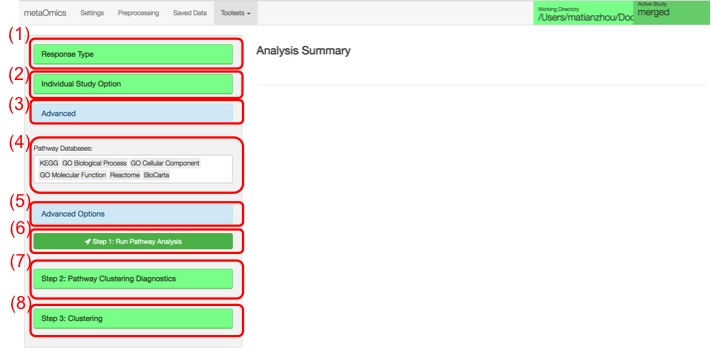
\includegraphics[scale=0.5]{./figure/metaPath/metaPathoption.pdf}
\caption{``MetaPath" options}
\label{fig:MetaPathoption}
\end{center}
\end{figure}

\textbf{Setup pathway analysis parameters:}
As shown in Figure~\ref{fig:MetaPathoption},
users need to specify {\color{red}(1)} whether the input gene expression profile is mixed of continuous data and discrete data;
{\color{red}(2)} response type, case/control labels (similar to MetaDE);
{\color{red}(3)} individual study option (similar to MetaDE);
{\color{red}(4)} advanced options including whether to adjust for covariates or the direction of hypothesis testing;.
In {\color{red}(5)}, users can select from 25 available pathway databases for the enrichment analysis.
In {\color{red}(6)}, users can select MetaPath method (either MAPE or CPI).
By default, the ``MAPE" approach is used. 
Other options include the pathway enrichment method (the Fisher's exact test or KS test), the minimum and maximum pathway size. If ``Fisher's exact test" is chosen for the enrichment method, users need to further specify the criteria for selection of DE genes, e.g. the number of top ranked genes. On the other hand, if ``KS test" is chosen, one needs to further specify whether to use permutation to obtain enrichment p-value. 

\begin{steps}
\item \textbf{Run Pathway Analysis:}
\label{step:metaPath1}
Once the above options are specified, users can click on {\color{red}(7)} to ``Run Pathway Analysis".

\item \textbf{Pathway clustering diagnostics:} 
\label{step:metaPath2}
From the previous step (\ref{step:metaPath1}), users can choose the top enriched pathways for further clustering. 
One can expand the drop-down menu and use FDR cutoff to choose top pathways and click on {\color{red}(8)} ``Pathway Clustering Diagnostics" to implement the second step.

\item \textbf{Pathway clustering with text mining:} 
\label{step:metaPath3}
From the previous step (\ref{step:metaPath2}), users can determine the optimal number of clusters in the pool of pathways selected. 
Now, one can specify the number of clusters and click on {\color{red}(9)} to get pathway ``Clustering" results. 
Note that you may not want to select too large $K$ since you wish to have a certain amount of pathways in each cluster for the validity of text mining algorithm. 
We generally suggest users to specify $K$ no larger than 7 for fewer than 100 pathways. 
\end{steps}




\subsubsection{Results}

\begin{figure}[H]
\begin{center}
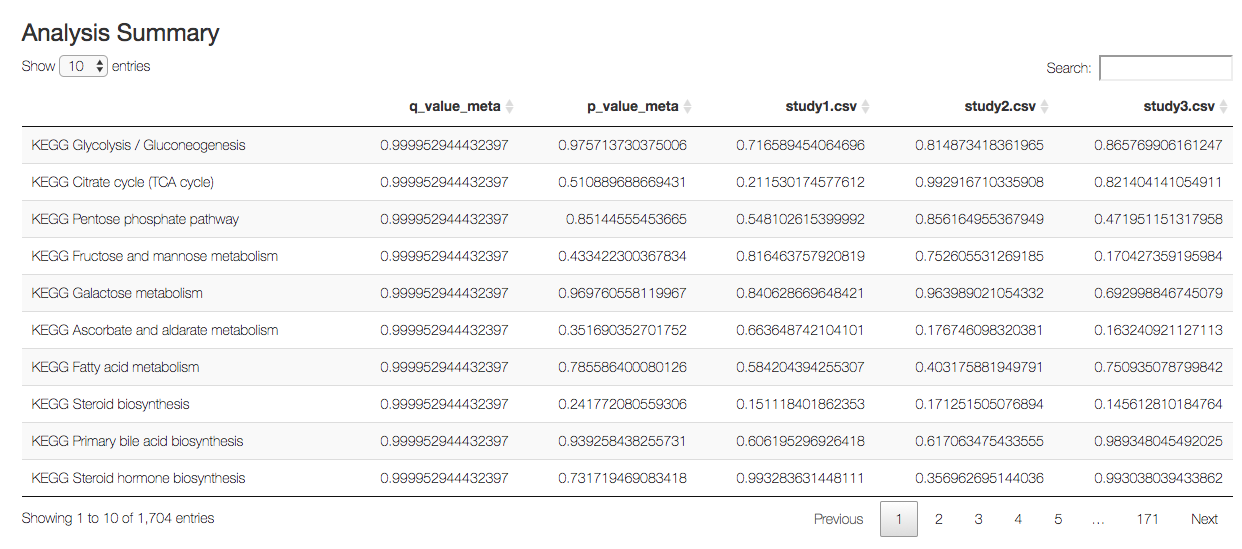
\includegraphics[scale=0.4]{./figure/metaPath/metaPathresult1.png}
\caption{``MetaPath" Results (1), 
this table shows analysis results of all pathways, 
including individual study association analysis p-value, meta pathway analysis p-value/FDR, etc. 
Users can sort these pathways by clicking the p\_value\_meta up arrow button.
In addition, users can search the pathway  name in the ``Search" bar.
}
\label{fig:MetaPathresult1}
\end{center}
\end{figure}

We used the AML data to demonstrate the usage of MetaPath module,
with the same filtering criteria and the phenotype of interest as in MetaDE module.
Detailed descriptions of these studies can be found in Table~\ref{tab:realDataLeukemia}. 
After \ref{step:metaPath1} is finished, a summary table was generated as shown in Figure~\ref{fig:MetaPathresult1} (based on the CPI method). 
The full table is automatically saved in the working directory specified before.  

\begin{figure}[H]
\begin{center}
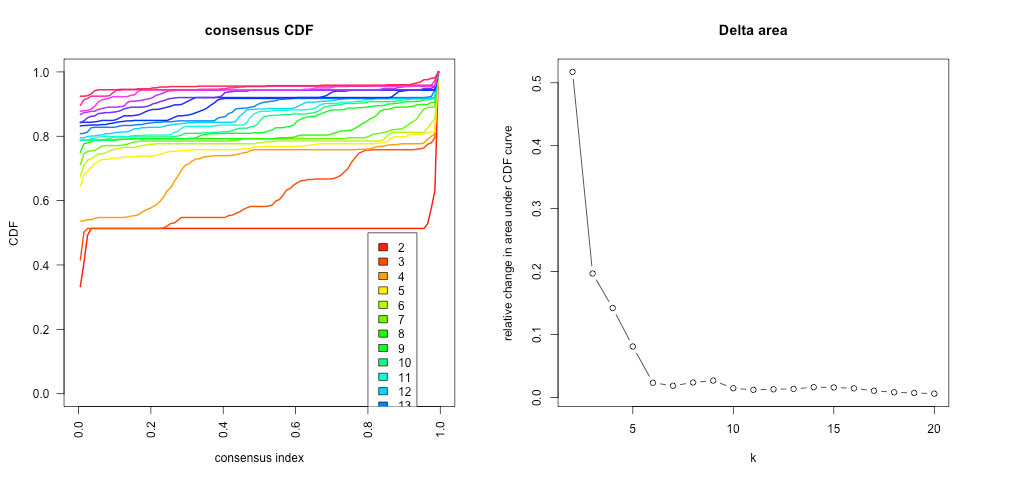
\includegraphics[scale=0.5]{./figure/metaPath/metaPathresult2.png}
\caption{``MetaPath" Results (2):
both plots assist users in finding the optimal number of clusters $K$ and users may refer to \cite{monti2003consensus} for detailed interpretation of the two plots. 
To be brief, the CDF of the consensus matrix for each $K$ (indicated by colors) is estimated by a histogram of 100 bins. 
The CDF reaches an approximate maximum implying consensus and cluster confidence is at a maximum at this $K$. 
The delta area shows the relative change in area under the CDF curve comparing $K$ and $K - 1$, thus allows users to determine $K$ at which there is no appreciable increase in CDF (which drops as the number of cluster increases).
In the example, $K=5$ is chosen since it locates at the elbow turning point (i.e. where the magnitude of incremental decrease in delta area diminishes).
}
\label{fig:MetaPathresult2}
\end{center}
\end{figure}

In order to perform pathway clustering analysis, we need to determine the number of clusters $K$.
By clicking ``Pathway Cluster Diagnostics" (\ref{step:metaPath2}), 
two plots are generated on the right panel (Figure \ref{fig:MetaPathresult2}): 
including a consensus CDF plot and a Delta area plot (both from the ``ConsensusClusterPlus" package). 
Note that in this specific example, we set FDR cutoff value in \ref{step:metaPath2} as 0.5, and 28 pathways left under this cutoff.
Both plots assist users in finding the optimal number of clusters $K$ and users may refer to \cite{monti2003consensus} for detailed interpretation of the two plots. 
To be brief, the CDF of the consensus matrix for each $K$ (indicated by colors) is estimated by a histogram of 100 bins. 
The CDF reaches an approximate maximum implying consensus and cluster confidence is at a maximum at this $K$. 
The delta area shows the relative change in area under the CDF curve comparing $K$ and $K - 1$, thus allows users to determine $K$ at which there is no appreciable increase in CDF (which drops as the number of cluster increases).
In the example, $K=5$ is chosen since it locates at the elbow turning point (i.e. where the magnitude of incremental decrease in delta area diminishes).

\begin{figure}[H]
\begin{center}
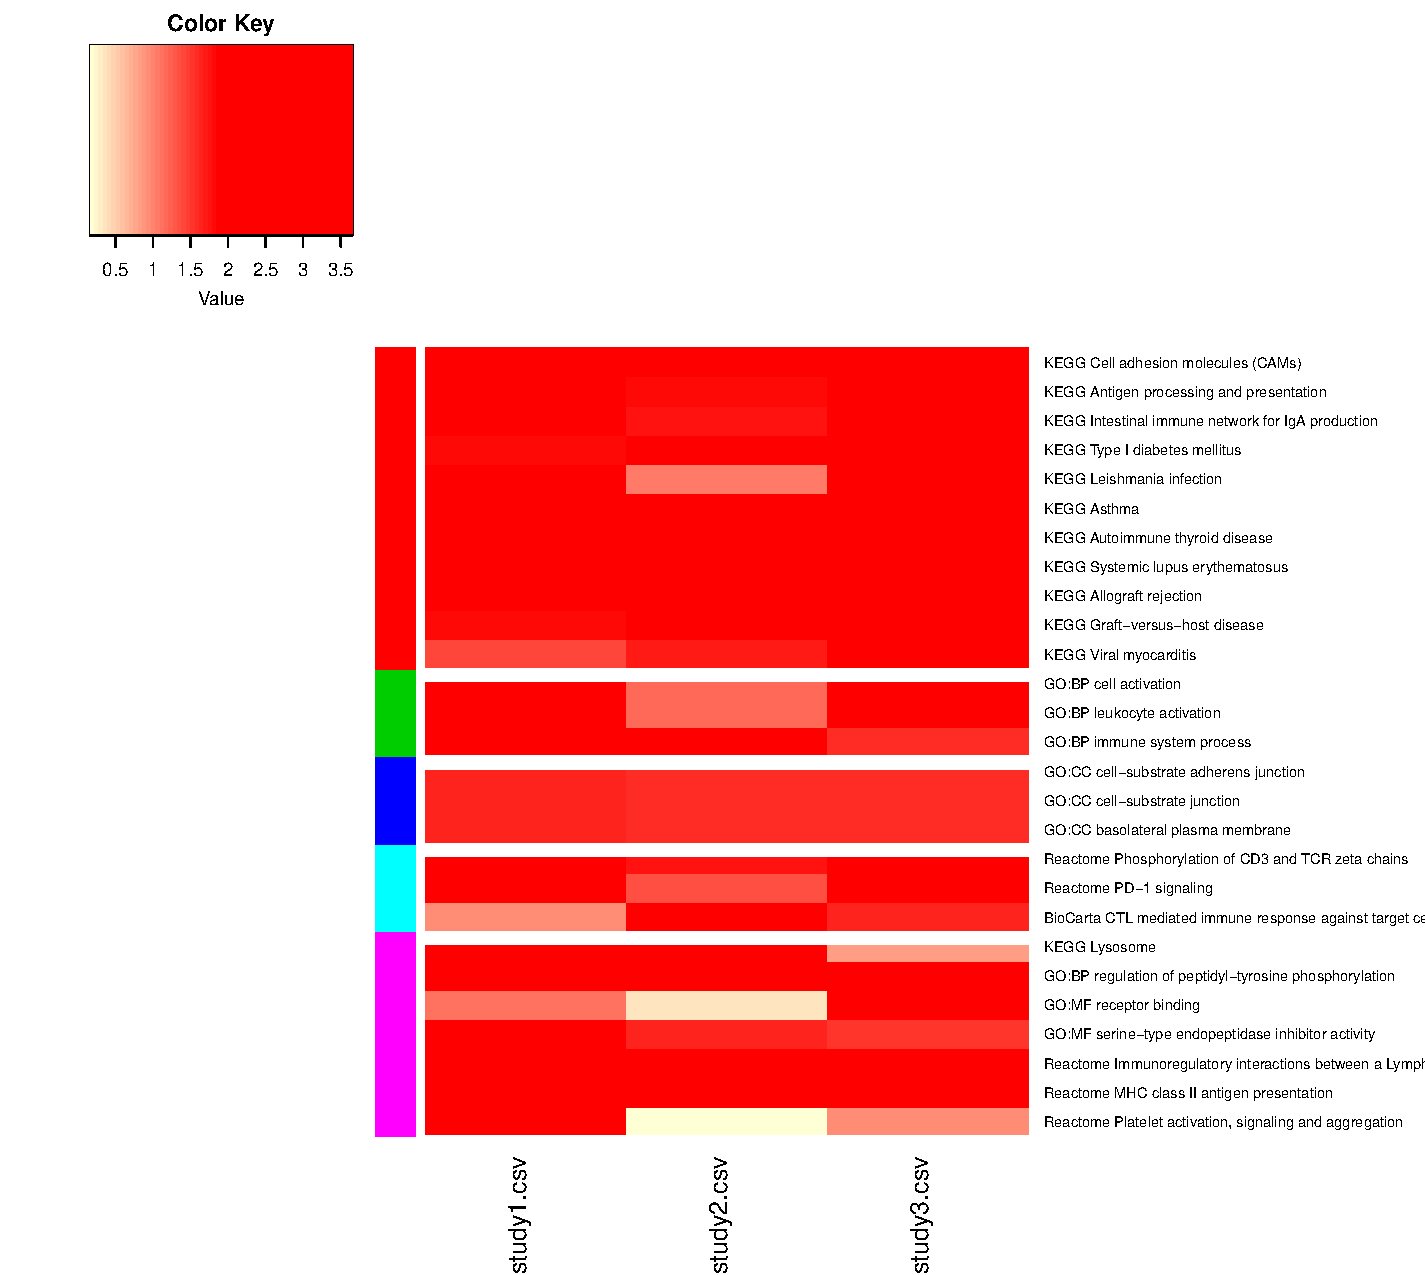
\includegraphics[scale=0.6]{./figure/metaPath/Heatmap_clusters_all.pdf}
\caption{``MetaPath" Results (3):
The heatmap in Figure~\ref{fig:MetaPathresult3} shows the -log10 transformed p-value of enrichment analysis in each study from \ref{step:metaPath1}. 
Studies are on columns and the selected pathways are on rows, red means more enriched. The pathways are sorted by the pathway clusters as indicated by the colors on the left side of the heatmap.}
\label{fig:MetaPathresult3}
\end{center}
\end{figure}


The heatmap in Figure~\ref{fig:MetaPathresult3} shows the -log10 transformed p-value of enrichment analysis in each study from \ref{step:metaPath1}. 
Studies are on columns and the selected pathways are on rows, red means more enriched. The pathways are sorted by the pathway clusters as indicated by the colors on the left side of the heatmap. 
In addition, 
key words of each cluster of pathways are extracted and analyzed by a built-in text mining algorithm and one file named ``Clustering\textunderscore Summary.csv" is saved to the working directory which shows a summary of the text mining results. 


